\setcounter{chapter}{2}
  	\chapter{Distribuzioni di probabilit\`{a} multidimensionali}
  	
  	\section{Probabilit\`{a} per variabili aleatorie in pi\`{u} \\ dimensioni}
  	
  	Quando un evento \`{e} identificato da un vettore $\underline{x}$, si parla di di distribuzioni di probabilit\`{a} multidimensionali o \textbf{joint pdf (probabilt\`{a} congiunta)}.  
  	
  	\begin{equation*}
  		pdf(\underline{x}): A \subseteq \mathbb{R}^n \rightarrow \mathbb{R}^+
  	\end{equation*}
  	
  	e la cdf per estensione della definizione mono-dimensionale \`{e}:
  	
	\begin{equation*}
  		cdf(\underline{x}) = \int_{A}pdf(\underline{x}) \cdot d\underline{x}
	\end{equation*}
  	
  	
	la probabili\`{a} di un evento per una variabile continua $\underline{x}$ \`{e} definita su una regione di spazio $A \subseteq \mathbb{R}^n$:
  	
	\vspace{0.2in}
  \begin{minipage}{0.5\textwidth}
		\begin{equation*}
  			P(\underline{x} \in A) = \int_{A}pdff(\underline{x}) \cdot d\underline{x}
  		\end{equation*}
  \end{minipage}
  \begin{minipage}{.4\textwidth}
    \centering
    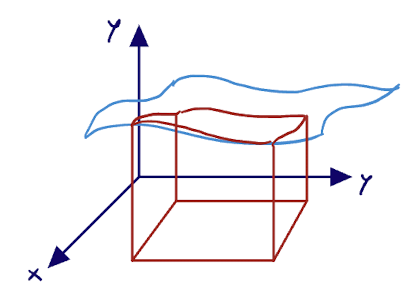
\includegraphics[scale = 0.42]{multi}

  \end{minipage}
	\vspace{0.2in}

Tale definizione di probabilit\`{a} verifica gli assiomi di Kolgomorov.
	
\section{Distribuzione di probabilit\`{a} marginale}

Data una distribuzione di probabilit\`{a} multidimensionale pdf($x_1,\cdots x_n)$ si definisce \textbf{distribuzione di probabilit\`{a} marginale}:

\begin{equation}
	f_{x_i}(x_1, \cdots,x_{i},\cdots,x_n) = \int pdf(x_1,\cdots,x_i,\cdots,x_n)dx_1\cdots dx_n
\end{equation}

 
\begin{figure}[ht]
\vspace{0.in}
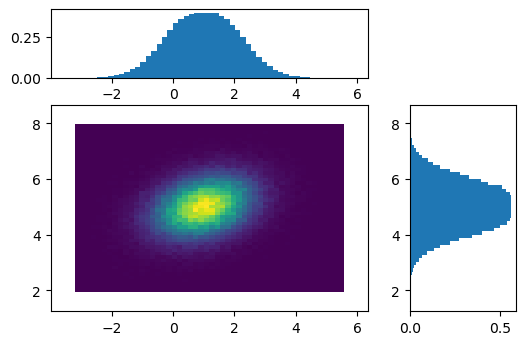
\includegraphics[scale = 0.6]{marginal.png}	
\centering
\vspace{0.in}
\caption{Distribuzione di probabilit\`{a} marginale per una pdf(x,y)}
\end{figure}

\subsubsection{Esempio}

Nel caso bi-dimensionale si ha che le rispettive distribuzioni marginali di una joint pdf$(x_1,x_2)$ sono date da:

\begin{equation}
	f_x(y) = \int pdf(x,y)dy \quad  \quad f_y(x) = \int pdf(x,y)dx
\end{equation}


\section{Distribuzione di probabilit\`{a} condizionata}

Per semplicit\`{a} consideriamo una distribuzione di probabilit\`{a} rispetto a due variabili aleatorie x ed y e le rispettive distribuzioni marginali $f_x$ e $f_y$. Vogliamo determinare la  probabilit\`{a} che $P(x \vert y = y_0)$ o $P(y \vert x = x_0) $. Consideriamo due eventi $A,B \subset \Omega$ disgiunti. Possiamo identificare le pdf come:

\begin{itemize}
	\item $P(A \cap B) \rightarrow $ joint pdf
	\item P(A) $\rightarrow$ pdf marginale
	\item $P(A|B) \rightarrow $ pdf condizionata
\end{itemize}

\noindent Definiamo L'evento A = $\{ y \; \vert \; x \in [x_0,x_0 +dx]\;,\; y \in \mathbb{R} \} $ e l'evento B = $\{ x \; \vert \; y \in [y_0,y_0 +dx]\;,\; x \in \mathbb{R} \} $. Le probabilit\`{a} associate ai singoli eventi sono P(A) = $f_x$ e P(B) = $f_y$. Mentre la probabilit\`{a} congiunta \`{e} $P(A \cap B) = \int pdf(x_0,y_0)dxdy$. 

Di conseguenza possiamo scrivere la probabilit\`{a} condizionata come:

\begin{equation}
	pdf(x \vert y = y_0) = P(A\vert B) = \dfrac{P(A \cap B)}{P(B)} = \dfrac{pdf(x,y_0)}{fx(y_0)}
\end{equation}

e analogamente:

\begin{equation}
	pdf(y \vert x = x_0) = \dfrac{pdf(x_0,y)}{f_y(x_0)}
\end{equation}

\section{Valore di aspettazione di una joint pdf}

Per una distribuzione di probabilit\`{a} congiunta abbiamo che il valore di aspettazione \`{e} definito da un vettore:
\begin{align}
E[\underline{x}] =
	\begin{bmatrix}
		\mu_x \\
		\mu_y \\
	\end{bmatrix}
	= 
	\begin{bmatrix}
		\int \int x \cdot pdf(x,y)dxdy \\
		\int \int y \cdot pdf(x,y)dxdy \\
	\end{bmatrix}	
\end{align}



\section{Varianza di una pdf multidimensionale}

Nel caso della Varianza, le componenti di una variabile aleatoria multidimensionale $\underline{x}$ possono essere legate tra loro, ovvero avere una relazione nel modo in cui variano, tale legame prende il nome di \textbf{covarianza}. Per due componenti $x_i$ e $x_j$ con $i \neq j$ si ha che: 

\begin{equation}
	\sigma_{i,j}^2 = E[(x_i - \mu_i)(x_j - \mu_j)] = E[x_ix_j] - E[x_i]E[x_j]
\end{equation}  	

\noindent mentre   	

\begin{equation}
	\sigma_{i,i}^2 = E[(x_i-\mu_i)^2]
\end{equation}
 
\noindent di conseguenza la varianza di una pdf($\underline{x})$ multidimensionale \`{e} rappresentata da una matrice che prende il nome di \textbf{matrice di covarianza} ed ha dimensione $n \times n$ nel caso $\underline{x}$ sia un vettore dimensione n.

\begin{equation}
	V[\underline{x}] = \begin{bmatrix}
		V[x_1] & \cdots \cdots	& Cov[x_1,x_n] \\
		\vdots & \ddots & \vdots \\
		Cov[x_n,x_1] & \cdots \cdots & V[x_n]
	\end{bmatrix}
\end{equation}
\newline

\noindent Nel caso in cui le componenti della variabile aleatoria $\underline{x}$ siano indipendenti tra loro si ha che la covarianza \`{e} nulla e dunque la (3.3) diventa una matrice diagonale.

\begin{equation}
	V[\underline{x}] = \begin{bmatrix}
		V[x_1] & \cdots \cdots	& 0 \\
		\vdots &\ddots & \vdots \\
		0 & \cdots \cdots & V[x_n]
	\end{bmatrix}
\end{equation}
\newline

La covarianza gode delle seguenti propriet\`{a}:
\begin{itemize}
	\item Avere $Cov[x_i,x_j] = 0 $ non implica necessariamente che le due variabili aleatorie siano statisticamente indipendenti.
	\item Se due variabili aleatorie sono statisticamente indipendenti \\ $\Rightarrow Cov[x_i,x_j] = 0 $
	\item Se due variabili aleatorie sono linearmente dipendenti \\$\Rightarrow Cov[x_i,x_j] = 0 $
	\item  La matrice di covarianza \`{e} simmetrica $\Rightarrow$ \`{e} diagonalizzabile.
\end{itemize}
 
 
\begin{figure}[ht]

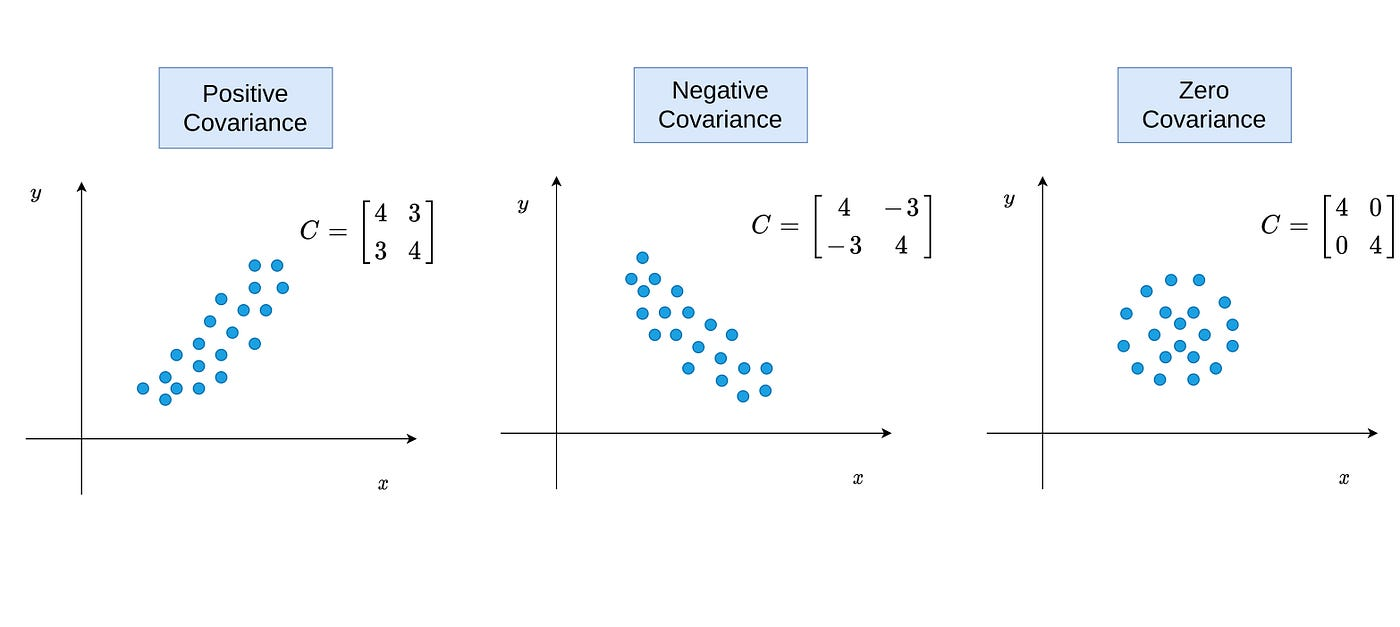
\includegraphics[scale = 0.23]{cov.jpeg}	
\centering
\caption{Esempi di come la covarianza si presenta in una distribuzione}
\end{figure} 

\section{Correlazione}
Gli elementi $V_{ij}$ della matrice di covarianza misurano il grado di correlazione tra le variabili $x_i$ e $x_j$. Dato che ogni variabili mostra una varianza finita e positiva \`{e} utile confrontare la covarianza  rispetto alle loro rispettive varianze, per farlo si introduce il coefficiente di correlazione:
\begin{equation}
	\rho_{ij} = \dfrac{Cov[x_i,x_j]}{\sigma_i \sigma_j}
\end{equation}

tale grandezza $\rho_{ij} \in [-1,1]$.

\begin{figure}[ht]
\vspace{0.2in}
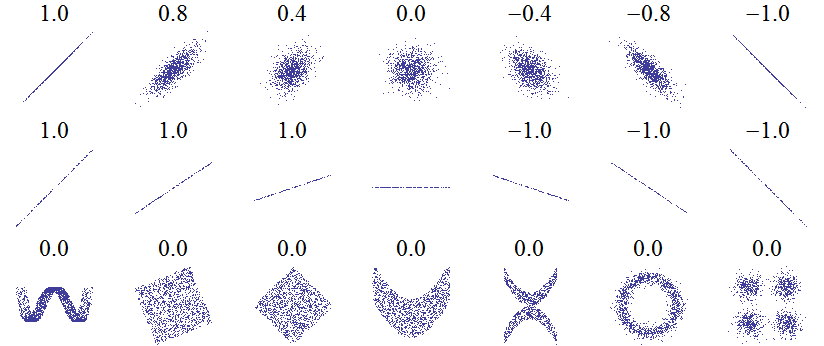
\includegraphics[scale = 0.45]{corre.png}	
\centering
\vspace{0.2in}
\caption{Indice di correlazione di Pearson per un campione di misure.}
\end{figure} 

\section{Variabili Statisticamente indipendenti}
Applichiamo la definizione di probabilit\`{a} congiunta data dall'equazione (3.3), poich\`{e} per ipotizziamo che  $P(x_2 \vert x_1)$ e $x_2$ non dipenda da $x_1$ avremo che:
\begin{equation*}
pdf(x_2 \vert x_1) = \dfrac{pdf(x_1,x_2)}{f_{x_1}} \Rightarrow pdf((x_1,x_2) = f_{x_1} \cdot pdf(x_2 \vert x_1)
\end{equation*}
si ha che  
\begin{equation*}
\quad f_{x_2}(x_1) = \int pdf(x_1,x_2)dx_1 = pdf(x_2\vert x_1) \int f_{x_1}dx_{1} = pdf (x_2 \vert x_1)
\end{equation*}
dunque si ha che:
\begin{equation*}
	pdf(x_1,x_2) = f_{x_1} \cdot f_{x_2}
\end{equation*}

\subsubsection{Definizione d'indipendenza}
Due variabili aleatorie $x_1$ ed $x_2$ descritte da una joint pdf($x_1,x_2)$ si definiscono \textbf{indipendenti} $\iff$ la joint pdf($x_1,x_2)$ = $pdf(x_1) \cdot pdf(x_2)$ dove $ pdf(x_1)$ e $pdf(x_2)$ coincidono con le marginali.

\subsubsection{Teorema}
Due variabili aleatorie $x_1$ ed $x_2$ descritte da una joint pdf($x_1,x_2)$ sono indipendenti $\Rightarrow$ la covarianza pu\`{o} essere scritta come:
\begin{equation}
	E[(x_1-\mu_{x_1})(x_2 - \mu_{x_2})] = E[(x_1-\mu_{x_1})] \cdot E[(x_2 - \mu_{x_2})]
\end{equation}
 
\section{Cambiamento di variabili per una pdf \\ multidimensionale}

La matrice della varianza (3.6) \`{e} diagonalizzabile, questo vuol dire che esiste un cambio di base che la diagonalizza, in fisica \`{e} equivalente ad avere un cambio di variabile. Sperimentalmente raccolto un campione di misure esiste sempre un cambio di variabile tale per cui la matrice di covarianza \`{e} diagonalizzabile. Anche se con un cambio di variabili le grandezze diventano decorrelate $Cov[x_i,x_j] = 0$ questo non vuol dire che siano statisticamente indipendenti.

Analogamente al caso mono-dimensionale per il cambio di variabili si ha che date delle funzioni:

\begin{align*}
	\begin{cases}
		x = u(\alpha,\beta)\\
		y = w(\alpha, \beta)
	\end{cases}
\end{align*}

la join pdf nelle nuove coordinate sar\`{a} data da:

\begin{equation}
	pdf(\alpha, \beta) = pdf(x,y) \cdot \vert detJ\vert
\end{equation}

dove J \`{e} la matrice Jacobiana associata alla trasformazione.
\subsection{Propagazione degli errori}

Ipotizziamo di avere un insieme di N misure $\{x_i\}_i^N$ e usiamo tali valori come componenti di un vettore $\underline{x} \in \mathbb{R}^N$, descritto da una pdf($\underline{x})$ di cui conosciamo $\underline{\mu}$ e matrice di covarianza $V[\underline{x}]$, vogliamo calcolare $y = u(\underline{x})$. Per Farlo approssimiamo u(\underline{x}) con un sviluppo di Taylor al primo ordine in un intorno di $\underline{\mu}$:

\begin{equation*}
	u(\underline{x}) \approx u(\underline{\mu})+ \nabla u\big \vert_{x = \mu}\cdot (\underline{x} - \underline{\mu})
\end{equation*}

\noindent Dunque i momenti della $pdf(\underline{y})$ sono:

\begin{itemize}
	\item E[y] = E[u($\underline{\mu}$)] + $\sum_{i =1}^{n} \dfrac{\partial}{\partial x_{i}}u(\underline{\mu})E[(x_i - \mu_{i})] = u(\underline{\mu}) $
	\item $\sigma_y^2 = E[y^2] - E[y]^2 = E[ (\underline{x} - \underline{\mu})^T H(u(\underline{x}))\big \vert_{x = \mu}(\underline{x} - \underline{\mu})] = \\ \\ =\sum_{i,j =1}^n \dfrac{\partial u(\underline{x})}{\partial x_i} \cdot \dfrac{\partial u(\underline{x})}{\partial x_j}\Big \vert_{x = \mu} \cdot V_{ij}$
\end{itemize}
\vspace{0.1in}
\noindent Per un caso bidimensionale l'incertezza su z = f(x,y) \`{e} data da:
\vspace{0.05in}
\begin{equation}
	\sigma_{z}^2 = \Big (\dfrac{\partial f(x,y)}{\partial x}\Big)^2 \Big \vert_{x =\mu}  \sigma_x^2 + \Big (\dfrac{\partial f(x,y)}{\partial y}\Big)^2\Big \vert_{x =\mu}  \sigma_y^2 + 2 \dfrac{\partial f(x,y)}{\partial x} \cdot \dfrac{\partial f(x,y)}{\partial y}\Big \vert_{x =\mu} Cov[x,y]
\end{equation}
\newpage

\subsection{Decorrelazione delle variabili}

Consideriamo un vettore $\underline{x}$ le cui componenti sono variabili aleatorie dipendenti tra loro. Poich\`{e} la matrice di covarianza \`{e} simmetrica possiamo definire una matrice $U$ che la diagonalizza $D[\underline{y}] = U^T V[\underline{x}]U$, tale matrice definisce un cambio di coordinate $\underline{y} = U\underline{x}$ dove le componenti di $\underline{y}$ risultano essere decorrelate tra loro.

\section{Distribuzione di Gauss Multidimensionale}

L'espressione di una Gaussiana in pi\`{u} dimensioni \`{e} data da:

\begin{equation}
	f(\underline{x} \; \big \vert \;  \underline{\mu},V) = \dfrac{1}{(2 \pi)^{\frac{n}{2}}detV^{\frac{1}{2}}} \cdot \exp{\Big [-\frac{1}{2} <(\underline{x} - \underline{\mu}),V^{-1}(\underline{x} - \underline{\mu})> \Big ]}
	\end{equation}
	
	
 
\begin{figure}[ht]
\vspace{0.1in}
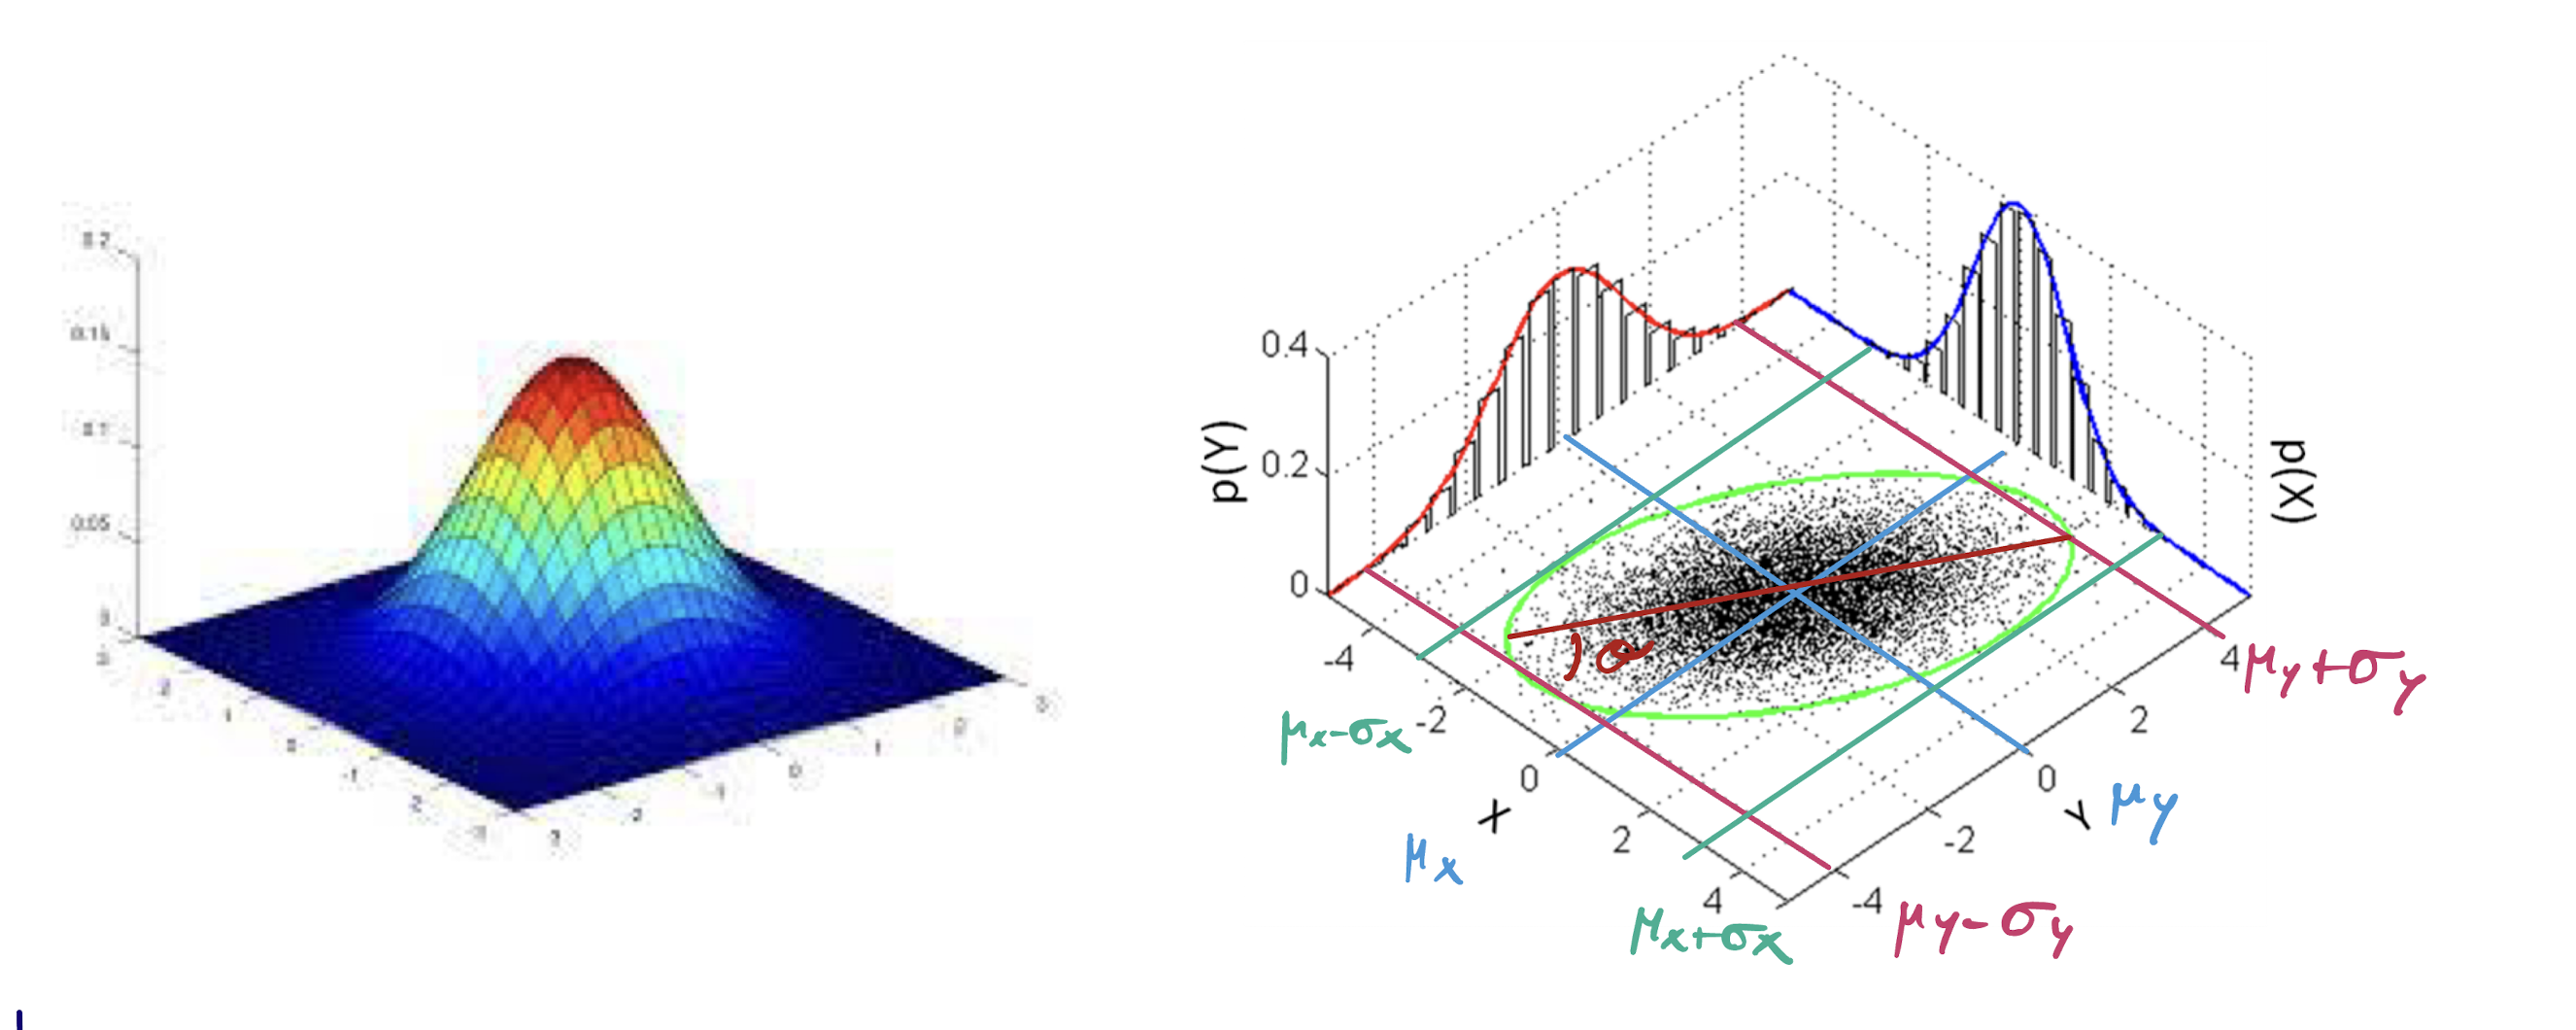
\includegraphics[scale = 0.3]{multiGauss}	
\centering
\vspace{0.1in}
\caption{Gaussiana in due variabili (x,y) e le sue distribuzioni marginali}
\end{figure}

\noindent La gaussiana in due dimensioni in generale ha un profilo ellittico per $1\sigma$. L'angolo d'inclinazione del semiasse maggiore \`{e} legato al coefficiente di correlazione:

\begin{equation}
	\theta = \dfrac{2\rho \sigma_x \sigma_y}{\sigma_x^2 - \sigma_y^2}
\end{equation}
\newline
Se esplicitiamo l'equazione (3.11) per due variabili si ha: 

\begin{align*}
	& f(x,y \; \big \vert \; \mu_x,\mu_y,V) = 
	\\
	\\
	&= \dfrac{1}{(2\pi)\sigma_x \sigma_y \sqrt{1-\rho^2}}  \exp{\Big \{ -\dfrac{1}{2(1-\rho^2)} \Big[ \Big ( \dfrac{x-\mu_x}{\sigma_x} \Big)^2 - \dfrac{2\rho(x-\mu_x)(y-\mu_y)}{\sigma_x \sigma_y} + \Big (\dfrac{y-\mu_y}{\sigma_y} \Big)^2  \Big]  \Big \}}	
\end{align*}
\newline
Se il coefficiente di correlazione di Pearson $\rho = 0$ possiamo riscrivere l'equazione precedente come:

\begin{align*}
	& f(x,y \; \big \vert \; \mu_x,\mu_y,V) = \dfrac{1}{(2\pi)\sigma_x \sigma_y} \exp{\Big \{ - \dfrac{1}{2} \Big[\Big ( \dfrac{x-\mu_x}{\sigma_x} \Big)^2 + \Big (\dfrac{y-\mu_y}{\sigma_y} \Big)^2 \Big] \Big \}} = 
	\\
	\\
	&\phantom{b= --------}= G(x,\mu_x,\sigma_x) \cdot G(y,\mu_y,\sigma_y)
\end{align*}
\newline
In generale \`{e} solo vero che due variabili statisticamente indipendenti sono anche decorrelate, nel caso Gaussiano vale anche il viceversa, ovvero se due variabili sono decorrelate allora sono anche statisticamente indipendenti.

\vspace{0.05cm}
\par\noindent\rule{\textwidth}{2pt}

\section{Capitolo 3 - Guida allo studio}

\begin{enumerate}
	\item 	Come sono definite le distribuzioni di probabilit\`{a} multi-dimensionali?
	\item Che cosa \`{e} una distribuzione di probabilit\`{a} marginale?
	\item Che cosa \`{e} una distribuzione di probabilit\`{a} condizionata?
	\item Che cosa \`{e} una distribuzione di probabilit\`{a} profilata?
	\item Cosa sono la covarianza ed il coefficiente di correlazione fra due variabili, data una distribuzione multi-dimensionale definita nel piano indicizzato dalle due variabili?
	\item Quale \`{e} la definizione di variabili indipendenti?
	\item Che relazione c'\`{e} fra l'indipendenza e la correlazione di due variabili?
	\item Come \`{e} scritta una Gaussiana a pi\`{u} dimensioni?
	\item Che cosa comporta una variazione del coefficiente di correlazione lineare, nella forma della distribuzione Gaussiana?
	\item Come si esprime il teorema di Bayes sfruttando la notazione delle distribuzioni di probabilit\`{a} continue a due variabili?
	\item Come si definiscono i momenti di distribuzioni multi-dimensionali?
	\item Come si possono ottenere variabili linearmente non correlate, a partire da un insieme di variabili e dalla loro distribuzione di probabilità congiunta?
	\item \`{E} necessario conoscere la distribuzione di probabilit\`{a} congiunta, per operare questa 	decorrelazione?
	\item Come si propagano le incertezze, in presenza di cambio di variabili?
	\item Che legame c'\`{e} fra la probabilit\`{a} e la statistica?

\end{enumerate}
